\section{Modelo Entidad Relación}
\subsection{Diseño}
A continuación se observa el modelo completo que diseñamos como solución al problema planteado.

\begin{figure}[h!]
  \centering
  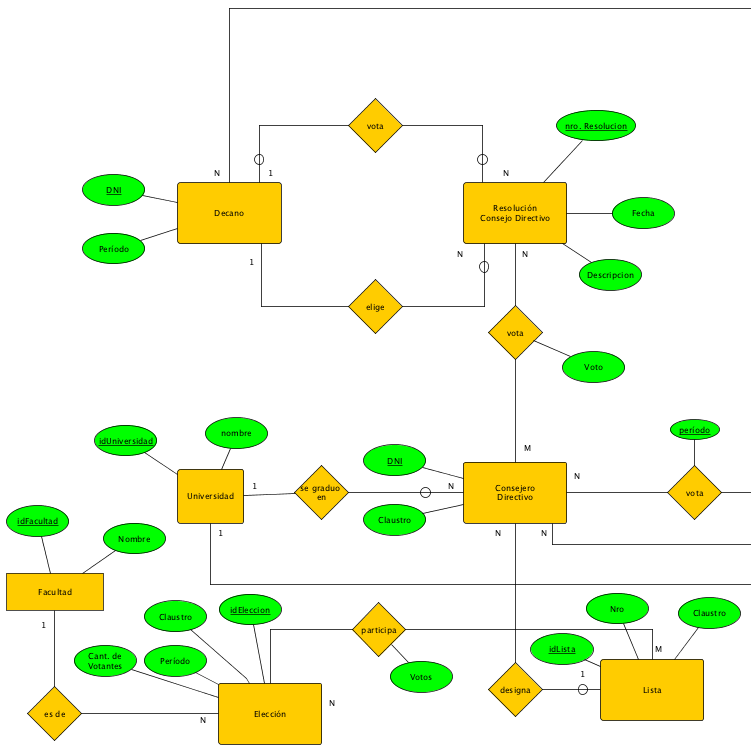
\includegraphics[width=0.9\textwidth]{./images/der1}
  \caption{Primera parte del Modelo Entidad Relación}
  \label{fig:clases4}
\end{figure}

\begin{figure}[h!]
  \centering
  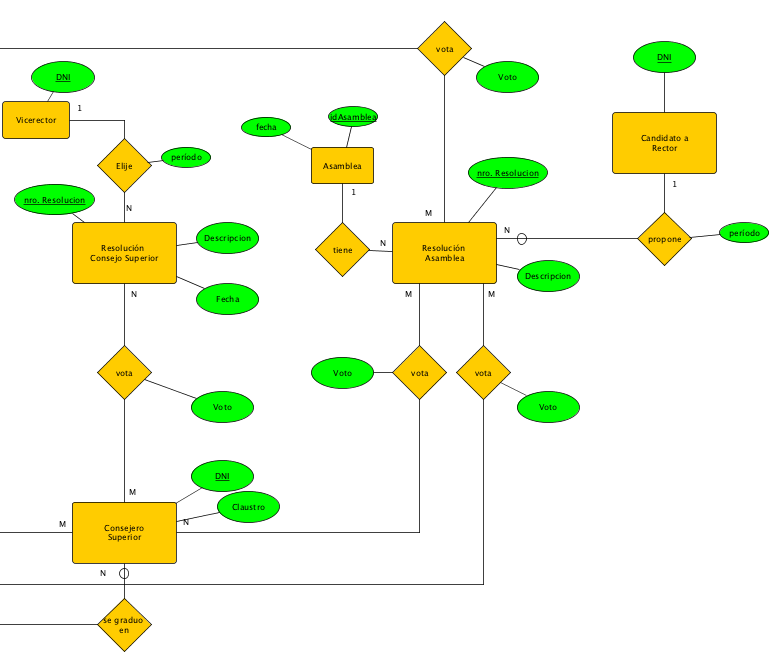
\includegraphics[width=1\textwidth]{./images/der2}
  \caption{Segunda parte del Modelo Entidad Relación}
  \label{fig:clases4}
\end{figure}
\newpage
\subsection{Consideraciones}
Estas son algunas consideraciones que tuvimos con respecto al enunciado del trabajo.

\begin{itemize}
\item  No es necesario tener la informacion de todos los integrantes de cada claustro ya que la votacion de consejeros directivos es secreta.
\item Al no modelar los integrantes de cada claustro no modelamos las condiciones que deben cumplir los candidatos a los diferentes cargos. Asumimos que las personas que estan cada una de esas tablas cumplen las condiciones.
\item No modelamos explicitamente cuando un candidato a rector es efectivamente elegido, sino que esta informacion se deduce de la cantidad de votos que recibio cada candidato. En este sentido tambien las elecciones de Rector que necesitaron mas de una votacion se deduce por las fechas en las que se junto la Asamblea a votar Rector y la cantidad de votos que saco cada uno.

\end{itemize}


\subsection{Restricciones}
Para que el modelo cumpla con lo estipulado en el estatuto, se deben tener en cuenta las siguientes restricciones:

\begin{itemize}
\item Una misma lista no puede estar en dos elecciones de distintas facultades.
\item Todas las resoluciones de Consejo Directivo son votadas por consejeros de la misma facultad.
\item M es 5 en la relación de votación de Consejero Directivo y Consejero Superior
\item Las resoluciones de Consejo Directivo son votadas por 4 Consejeros estudiantiles, 4 graduados y 8 profesores, correspondientes a la facultad y período de la resolución.
\item La composición del Consejo Directivo cumple lo especificado en el estatuto (por ejemplo para estudiantes,3 para la mayoría y 1 para la primer minoría si llega al 20\% de los votos).  

\end{itemize}

\subsection{Modelo Relacional}
Este es el MR correspondiente a MER presentado anteriormente. En él se pueden ver las distintas tablas necesarias para realizar la implementación.


\noindent \textbf{Decano}(\underline{DNI}, Periodo) \\
\textbf{ResolucionConsejoDirectivo}(\underline{nroResolucion}, Fecha, \dashuline{idDecanoQueVota}, \\\dashuline{idDecanoElegido})\\
\textbf{ResolucionConsejoSuperior}(\underline{nroResolucion}, Fecha)\\
\textbf{Asamblea}(\underline{idAsamblea}, fecha)\\
\textbf{ResolucionAsamblea}(\underline{nroResolucion}, \dashuline{idAsamblea, idCandidatoRector, idCandidatoVicerrector})\\
\textbf{CandidatoARector}(\underline{DNI}, periodo)\\
\textbf{Universidad}(\underline{idUniversidad}, nombre)\\
\textbf{ConsejeroDirectivo}(\underline{DNI}, Claustro, \dashuline{idUniversidad, idLista})\\
\textbf{ConsejeroSuperior}(\underline{DNI})\\
\textbf{Lista}(\underline{idLista}, Nro, Claustro)\\
\textbf{Facultad}(\underline{idFacultad}, Nombre)\\
\textbf{Eleccion}(\underline{idEleccion}, Periodo, CantDeVolantes, \dashuline{idFacultad})\\
\textbf{CandidatoAVicerrector}(\underline{DNI})\\
\textbf{VotaDecanoAsamblea}(\underline{idDecano, nroResolucion}, voto)\\
\textbf{VotaSuperiorAsamblea}(\underline{DNI}, voto)\\
\textbf{VotaDirectivoAsamblea}(\underline{DNI}, voto)\\
\textbf{VotaResolucionDirectivo}(\underline{DNI, nroResolucion}, voto)\\
\textbf{VotaResolucionSuperior}(\underline{DNI, nroResolucion}, voto)\\
\textbf{VotaDirectivoSuperior}(\underline{DNI\_Directivo, DNI\_Superior, periodo})\\
\textbf{Participa}(\underline{idLista, idEleccion})\\
